%% LICENCE: CC-BY-NC-SA
%% Copyright: Jesús Espino
\documentclass[10pt]{beamer}

\usepackage[utf8]{inputenc}
\usepackage[spanish]{babel}
\usepackage{graphicx}

\mode<presentation>
\usetheme{Madrid}
%\usecolortheme[RGB={111,73,135}]{structure}
\usecolortheme[RGB={128,0,0}]{structure}
%\usecolortheme[RGB={0,96,0}]{structure}
%\usecolortheme[RGB={200,0,200}]{structure}
%\usecolortheme[RGB={0,128,0}]{structure}
%\usecolortheme[RGB={0,0,128}]{structure}
\usefonttheme{serif}
\useinnertheme{rectangles}
\useoutertheme{split}

\setbeamercovered{transparent}

\title{Objetos en CPython}
\author{Jesús Espino García}
\date{24 de Noviembre de 2013}
\subject{Objetos en CPython}

\institute[Kaleidos]{jesus.espino@kaleidos.net\\@jespinog\\
\includegraphics[height=1.5cm]{img/pycones.png}
\includegraphics[height=1.5cm]{img/kaleidos.png}}

\setcounter{tocdepth}{2}

\AtBeginSubsection[]
{
  \begin{frame}[containsverbatim]<beamer>{Indice}
    \tableofcontents[sectionstyle=show/shaded,subsectionstyle=show/shaded/hide]
  \end{frame}
}

\begin{document}

  \frame{\maketitle}

  \section*{Introducción}

  \begin{frame}[containsverbatim]
    \frametitle{Introducción}
    \begin{itemize}
      \item Python 3.3
      \item Usaré ctypes para los ejemplos.
      \item La estructura de un objeto en cpython.
      \item Los objetos escritos en c de python.
      \item El proceso de creación de un nuevo objeto.
    \end{itemize}
  \end{frame}

  \section*{Definiciones}

  \begin{frame}[containsverbatim]
    \frametitle{¿Qué es un tipo en python?}
    \begin{itemize}
      \item Un tipo es una clase
      \item Es una estructura compuesta de datos y slots
      \item Los slots son punteros a funciones que definen comportamientos
      \item Los tipos son objetos de python
      \item Los tipos son de objetos de tipo tipo
    \end{itemize}
  \end{frame}

  \begin{frame}[containsverbatim]
    \frametitle{¿Qué es un tipo en python?}
    \begin{verbatim}
>>> class Prueba:
...   pass
...
>>> type(Prueba)
<class 'type'>
>>> isinstance(Prueba, object)
True
>>> isinstance(type, object)
True
>>> type(type)
<class 'type'>
    \end{verbatim}
  \end{frame}

  \begin{frame}[containsverbatim]
    \frametitle{¿Qué es una instancia?}
    \begin{itemize}
      \item Es exactamente lo mismo que un objeto.
      \item Es una zona reservada de la memoria con datos.
      \item Tiene un tipo (y solo 1) que determina qué puede hacer el objeto.
      \item El tipo de un objeto no cambia a lo largo de su vida (existen excepciones).
    \end{itemize}
  \end{frame}

  \begin{frame}[containsverbatim]
    \frametitle{¿Qué es una instancia?}
    \begin{verbatim}
>>> prueba = Prueba()
>>> type(prueba)
<class '__main__.Prueba'>
>>> prueba
<__main__.Prueba object at 0x7f3555af9bd0>
>>> Prueba
<class '__main__.Prueba'>
>>> id(prueba)
139867047566288
>>> hex(id(prueba))
'0x7f3555af9bd0'
    \end{verbatim}
  \end{frame}

  \begin{frame}[containsverbatim]
    \frametitle{Diagrama de herencia}
    \begin{center}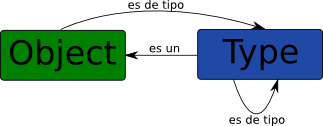
\includegraphics[width=6cm]{img/Object-Type-Relation.png}\end{center}
  \end{frame}

  \begin{frame}[containsverbatim]
    \frametitle{Diagrama de herencia}
    \begin{center}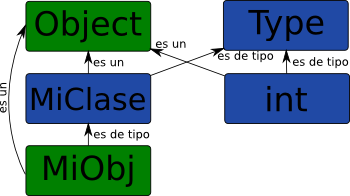
\includegraphics[width=6cm]{img/MyClass-BuiltinClass-Relation.png}\end{center}
  \end{frame}

  \begin{frame}[containsverbatim]
    \frametitle{Diagrama de herencia}
    \begin{center}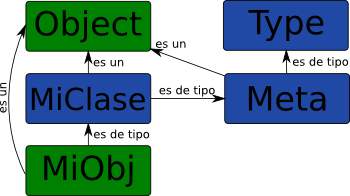
\includegraphics[width=6cm]{img/Metaclass-Relation.png}\end{center}
  \end{frame}

  \section*{Estructura de objetos}

  \begin{frame}[containsverbatim]
    \frametitle{Estructura básica de un objetos}
    \begin{center}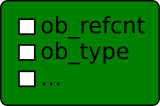
\includegraphics[width=4cm]{img/PyObject.png}\end{center}
    \begin{itemize}
      \item \verb+ob_refcnt+: contador de referencias
      \item \verb+ob_type+: puntero al tipo de datos
      \item Otros datos específicos para este tipo
    \end{itemize}
  \end{frame}

  \begin{frame}[containsverbatim]
    \frametitle{Estructura variable básica de un objetos}
    \begin{center}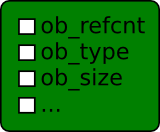
\includegraphics[width=4cm]{img/PyVarObject.png}\end{center}
    \begin{itemize}
      \item \verb+ob_refcnt+: contador de referencias
      \item \verb+ob_type+: puntero al tipo de datos
      \item \verb+ob_size+: tamaño del objeto
      \item Otros datos específicos para este tipo
    \end{itemize}
  \end{frame}

  \section*{Tipos en CPython}

  \begin{frame}[containsverbatim]
    \frametitle{El objeto None}
    \begin{center}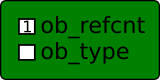
\includegraphics[width=4cm]{img/None.png}\end{center}
    \begin{itemize}
      \item Es el tipo más simple
      \item Su instancia es singleton
      \item No añade ningún dato extra a la estructura básica de objeto
    \end{itemize}
  \end{frame}

  \begin{frame}[containsverbatim]
    \frametitle{Very bad things}
    \begin{verbatim}
>>> ref_cnt = ctypes.c_long.from_address(id(None))
>>> ref_cnt.value = 0
Fatal Python error: deallocating None

Current thread 0x00007f2fb8d2a700:
  File "<stdin>", line 1 in <module>
[2]    10960 abort (core dumped)  python3
    \end{verbatim}
  \end{frame}

  \begin{frame}[containsverbatim]
    \frametitle{El objeto int}
    \begin{center}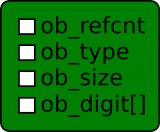
\includegraphics[width=4cm]{img/Int.png}\end{center}
    \begin{itemize}
      \item \verb+ob_digit+: array de enteros
      \item El valor del entero es \verb+sum(map(lambda x: 1024*1024*1024, ob_size))+
    \end{itemize}
  \end{frame}

  \begin{frame}[containsverbatim]
    \frametitle{El objeto int}
    \begin{center}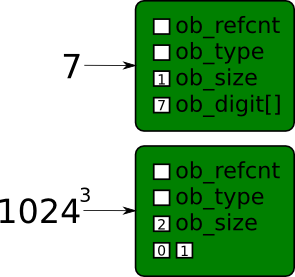
\includegraphics[width=6cm]{img/Int-Usage.png}\end{center}
  \end{frame}

  \begin{frame}[containsverbatim]
    \frametitle{El objeto int}
    \begin{verbatim}
>>> longsize = ctypes.sizeof(ctypes.c_long)
>>> intsize = ctypes.sizeof(ctypes.c_int)
>>> x = 100
>>> ctypes.c_long.from_address(id(x) + longsize * 2)
c_long(1)
>>> ctypes.c_uint.from_address(id(x) + longsize * 3)
c_uint(100)
>>> x = 1024 * 1024 * 1024
>>> ctypes.c_long.from_address(id(x) + longsize * 2)
c_long(2)
>>> ctypes.c_uint.from_address(id(x) + longsize * 3)
c_uint(0)
>>> ctypes.c_uint.from_address(id(x) + longsize * 3 + intsize)
c_uint(1)
    \end{verbatim}
  \end{frame}

  \begin{frame}[containsverbatim]
    \frametitle{Very bad things}
    \begin{verbatim}
>>> longsize = ctypes.sizeof(ctypes.c_long)
>>> x = 1000
>>> int_value = ctypes.c_uint.from_address(id(x) + longsize * 3)
>>> int_value.value = 1001
>>> x
1001
>>> 1000
1000
    \end{verbatim}
  \end{frame}

  \begin{frame}[containsverbatim]
    \frametitle{Very bad things}
    \begin{verbatim}
>>> longsize = ctypes.sizeof(ctypes.c_long)
>>> x = 100
>>> int_value = ctypes.c_uint.from_address(id(x) + longsize * 3)
>>> int_value.value = 101
>>> x
101
>>> 100
101
>>> 100 + 2
103
    \end{verbatim}
  \end{frame}

  \begin{frame}[containsverbatim]
    \frametitle{El objeto bool}
    \begin{center}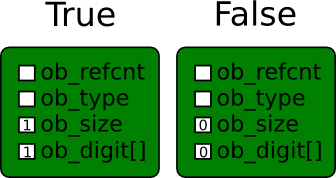
\includegraphics[width=6cm]{img/True-False.png}\end{center}
    \begin{itemize}
      \item Realmente son 2 instancias int con un tipo específico y valores 0 y 1
    \end{itemize}
  \end{frame}

  \begin{frame}[containsverbatim]
    \frametitle{El objeto bool}
    \begin{verbatim}
>>> longsize = ctypes.sizeof(ctypes.c_long)
>>> ctypes.c_long.from_address(id(True) + longsize * 2)
c_long(1)
>>> ctypes.c_uint.from_address(id(True) + longsize * 3)
c_uint(1)
>>> ctypes.c_long.from_address(id(False) + longsize * 2)
c_long(0)
>>> ctypes.c_uint.from_address(id(False) + longsize * 3)
c_uint(0)
    \end{verbatim}
  \end{frame}

  \begin{frame}[containsverbatim]
    \frametitle{Very bad things}
    \begin{verbatim}
>>> val = ctypes.c_int.from_address(id(True) + longsize * 2)
>>> val.value = 0
>>> val = ctypes.c_int.from_address(id(True) + longsize * 3)
>>> val.value = 0
>>> True == False
True
    \end{verbatim}
  \end{frame}

  \begin{frame}[containsverbatim]
    \frametitle{El objeto float}
    \begin{center}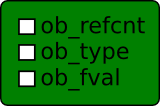
\includegraphics[width=4cm]{img/Float.png}\end{center}
    \begin{itemize}
      \item \verb+ob_fval+: es un double
    \end{itemize}
  \end{frame}

  \begin{frame}[containsverbatim]
    \frametitle{El objeto float}
    \begin{verbatim}
>>> longsize = ctypes.sizeof(ctypes.c_long)
>>> x = 1.5
>>> ctypes.c_double.from_address(id(x) + longsize * 2)
c_double(1.5)
    \end{verbatim}
  \end{frame}

  \begin{frame}[containsverbatim]
    \frametitle{El objeto complex}
    \begin{center}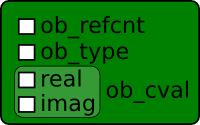
\includegraphics[width=4cm]{img/Complex.png}\end{center}
    \begin{itemize}
      \item \verb+cval+: dos valores double \verb+real+ e \verb+imag+
    \end{itemize}
  \end{frame}

  \begin{frame}[containsverbatim]
    \frametitle{El objeto complex}
    \begin{verbatim}
>>> longsize = ctypes.sizeof(ctypes.c_long)
>>> doublesize = ctypes.sizeof(ctypes.c_double)
>>> x = 1 + 3j
>>> ctypes.c_double.from_address(id(x) + longsize * 2)
c_double(1.0)
>>> ctypes.c_double.from_address(id(x) + longsize * 2 + doublesize)
c_double(3.0)
    \end{verbatim}
  \end{frame}

  \begin{frame}[containsverbatim]
    \frametitle{El objeto bytes}
    \begin{center}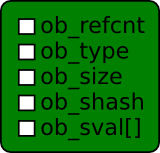
\includegraphics[width=4cm]{img/Bytes.png}\end{center}
    \begin{itemize}
      \item \verb+ob_shash+: hash de la cadena o -1
      \item \verb+ob_sval+: cadena terminada en \\0 (tipo C)
    \end{itemize}
  \end{frame}


  \begin{frame}[containsverbatim]
    \frametitle{El objeto bytes}
    \begin{center}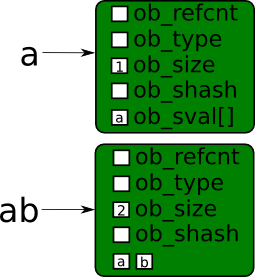
\includegraphics[width=5cm]{img/Bytes-Usage.png}\end{center}
  \end{frame}

  \begin{frame}[containsverbatim]
    \frametitle{El objeto bytes}
    \begin{verbatim}
>>> longsize = ctypes.sizeof(ctypes.c_long)
>>> charsize = ctypes.sizeof(ctypes.c_char)
>>> x = b"yep"
>>> ctypes.c_long.from_address(id(x) + longsize * 2)
c_long(3)
>>> hash(x)
954696267706832433
>>> ctypes.c_long.from_address(id(x) + longsize * 3)
c_long(954696267706832433)
>>> ctypes.c_char.from_address(id(x) + longsize * 4)
c_char(b'y')
>>> ctypes.c_char.from_address(id(x) + longsize * 4 + charsize)
c_char(b'e')
>>> ctypes.c_char.from_address(id(x) + longsize * 4 + charsize * 2)
c_char(b'p')
>>> ctypes.c_char.from_address(id(x) + longsize * 4 + charsize * 3)
c_char(b'\x00')
    \end{verbatim}
  \end{frame}


  \begin{frame}[containsverbatim]
    \frametitle{El objeto bytearray}
    \begin{center}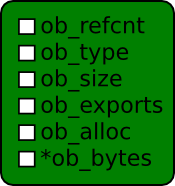
\includegraphics[width=4cm]{img/Bytearray.png}\end{center}
    \begin{itemize}
      \item \verb+ob_exports+: memoryviews apuntando a este objeto
      \item \verb+ob_alloc+: contabiliza el número de bytes almacenados
      \item \verb+ob_bytes+: puntero a la posición de los bytes almacenados
    \end{itemize}
  \end{frame}

  \begin{frame}[containsverbatim]
    \frametitle{El objeto bytearray}
    \begin{verbatim}
>>> longsize = ctypes.sizeof(ctypes.c_long)
>>> charsize = ctypes.sizeof(ctypes.c_char)
>>> x = bytearray(b"yep")
>>> ctypes.c_long.from_address(id(x) + longsize * 2)
c_long(3)
>>> ctypes.c_long.from_address(id(x) + longsize * 3)
c_long(0)
>>> ctypes.c_long.from_address(id(x) + longsize * 4)
c_char(4)
>>> addr = ctypes.c_void_p.from_address(id(x) + longsize * 5).value
>>> ctypes.c_char.from_address(addr)
c_char(b'y')
>>> ctypes.c_char.from_address(addr + charsize)
c_char(b'e')
    \end{verbatim}
  \end{frame}

  \begin{frame}[containsverbatim]
    \frametitle{El objeto tuple}
    \begin{center}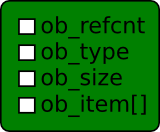
\includegraphics[width=4cm]{img/Tuple.png}\end{center}
    \begin{itemize}
      \item \verb+ob_item+: array de punteros a PyObject
    \end{itemize}
  \end{frame}

  \begin{frame}[containsverbatim]
    \frametitle{El objeto tuple}
    \begin{verbatim}
>>> longsize = ctypes.sizeof(ctypes.c_long)
>>> x = (True, False)
>>> ctypes.c_long.from_address(id(x) + longsize * 2)
c_long(2)
>>> ctypes.c_void_p.from_address(id(x) + longsize * 3)
c_void_p(140048684311616)
>>> ctypes.c_void_p.from_address(id(x) + longsize * 4)
c_void_p(140048684311648)
>>> id(True)
140048684311616
>>> id(False)
140048684311648
    \end{verbatim}
  \end{frame}

  \begin{frame}[containsverbatim]
    \frametitle{Very Bad Things}
    \begin{verbatim}
>>> longsize = ctypes.sizeof(ctypes.c_long)
>>> x = (1, 2, 3)
>>> tuple_size = ctypes.c_long.from_address(id(x) + longsize * 2)
>>> tuple_size.value = 2
>>> x
(1, 2)
    \end{verbatim}
  \end{frame}

  \begin{frame}[containsverbatim]
    \frametitle{El objeto lista}
    \begin{center}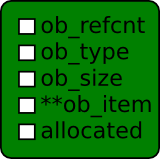
\includegraphics[width=4cm]{img/List.png}\end{center}
    \begin{itemize}
      \item \verb+ob_item+: puntero a punteros de PyObject
      \item \verb+allocated+: memoria reservada actualmente para la lista
    \end{itemize}
  \end{frame}

  \begin{frame}[containsverbatim]
    \frametitle{El objeto lista}
    \begin{verbatim}
>>> longsize = ctypes.sizeof(ctypes.c_long)
>>> x = [1,2,3]
>>> ctypes.c_long.from_address(id(x) + longsize * 2)
c_long(3)
>>> ctypes.c_void_p.from_address(id(x) + longsize * 3)
c_void_p(36205328)
>>> ctypes.c_void_p.from_address(36205328)
c_void_p(140048684735040)
>>> id(1)
140048684735040
>>> ctypes.c_void_p.from_address(36205328 + longsize)
c_void_p(140048684735072)
>>> id(2)
140048684735072
    \end{verbatim}
  \end{frame}

  \begin{frame}[containsverbatim]
    \frametitle{Very Bad Things}
    \begin{verbatim}
>>> longsize = ctypes.sizeof(ctypes.c_long)
>>> x = [1,2,3,4,5,6,7,8,9,10]
>>> y = [10,9,8,7]
>>> datos_y = ctypes.c_long.from_address(id(y) + longsize * 3)
>>> datos_x = ctypes.c_long.from_address(id(x) + longsize * 3)
>>> datos_y.value = datos_x.value
>>> y
[1, 2, 3, 4]
>>> x[0] = 7
>>> y
[7, 2, 3, 4]
    \end{verbatim}
  \end{frame}

  \begin{frame}[containsverbatim]
    \frametitle{El objeto dict}
    \begin{center}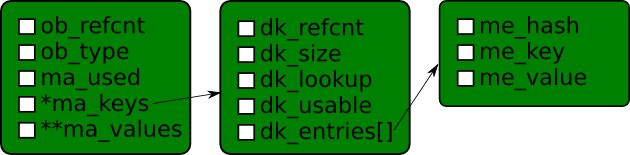
\includegraphics[width=9cm]{img/Dict.png}\end{center}
    \begin{itemize}
      \item \verb+ma_used+: número de items.
      \item \verb+ma_keys+: puntero a la estructura que almacena el diccionario.
      \item \verb+ma_values+: puntero a punteros de PyObject (para slited tables y NULL para combined tables).
    \end{itemize}
  \end{frame}

  \begin{frame}[containsverbatim]
    \frametitle{PyDictKeysObject}
    \begin{center}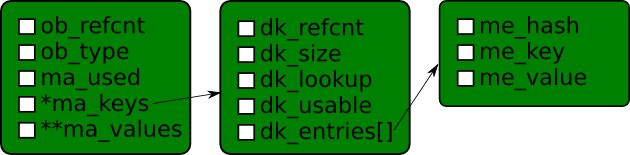
\includegraphics[width=9cm]{img/Dict.png}\end{center}
    \begin{itemize}
      \item \verb+dk_refcnt+: contador de referencias
      \item \verb+dk_size+: Tamaño total de la tabla hash para guardar entradas
      \item \verb+dk_lookup+: Slot para función de búsqueda
      \item \verb+dk_usable+: La fracción usable del diccionario antes de un redimensionado
      \item \verb+dk_entries[n]+: Las entradas en la tabla hash
    \end{itemize}
  \end{frame}

  \begin{frame}[containsverbatim]
    \frametitle{PyDictKeyEntry}
    \begin{center}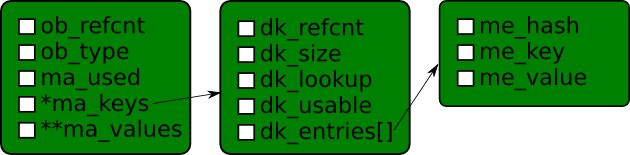
\includegraphics[width=9cm]{img/Dict.png}\end{center}
    \begin{itemize}
      \item \verb+me_hash+: Hash de la key
      \item \verb+me_key+: Puntero al objeto key
      \item \verb+me_value+: Puntero al objeto valor (Solo para combined tables)
    \end{itemize}
  \end{frame}

  \begin{frame}[containsverbatim]
    \frametitle{El objeto dict}
    \begin{verbatim}
>>> longsize = ctypes.sizeof(ctypes.c_long)
>>> d = {1: 3, 7: 5}
>>> keys = ctypes.c_void_p.from_address(id(d) + longsize * 3).value
>>> keyentry1 = keys + longsize * 4 + longsize * hash(1) * 3
>>> keyentry7 = keys + longsize * 4 + longsize * hash(7) * 3
>>> key1 = ctypes.c_long.from_address(keyentry1 + longsize).value
>>> val1 = ctypes.c_long.from_address(keyentry1 + longsize * 2).value
>>> key7 = ctypes.c_long.from_address(keyentry7 + longsize).value
>>> val7 = ctypes.c_long.from_address(keyentry7 + longsize * 2).value
>>> ctypes.c_uint.from_address(key1 + longsize * 3)
c_long(1)
>>> ctypes.c_uint.from_address(val1 + longsize * 3)
c_long(3)
>>> ctypes.c_uint.from_address(key7 + longsize * 3)
c_long(7)
>>> ctypes.c_uint.from_address(val7 + longsize * 3)
c_long(5)
    \end{verbatim}
  \end{frame}

  \begin{frame}[containsverbatim]
    \frametitle{El objeto type (no completo)}
    \begin{itemize}
      \item \verb+tp_name+: Nombre de la clase
      \item \verb+tp_doc+: El docstring del tipo
      \item \verb+tp_dict+: El diccionario de attributos del tipo
      \item \verb+tp_dictoffset+: El offset al diccionario de atributos de los objetos
      \item \verb+tp_as_number+: Puntero a estructura de slots
      \item \verb+tp_as_sequence+: Puntero a estructura de slots
      \item \verb+tp_as_mappings+: Puntero a estructura de slots
    \end{itemize}
  \end{frame}

  \begin{frame}[containsverbatim]
    \frametitle{El objeto type}
    \begin{verbatim}
>>> longsize = ctypes.sizeof(ctypes.c_long)
>>> ctypes.c_char_p.from_address(id(int) + longsize * 3)
'int'
>>> ctypes.c_char_p.from_address(id(type) + longsize * 3)
'type'
>>> class Prueba:
...     pass
...
>>> ctypes.c_char_p.from_address(id(Prueba) + longsize * 3)
'Prueba'
    \end{verbatim}
  \end{frame}

  \begin{frame}[containsverbatim]
    \frametitle{Very Bad Things}
    \begin{verbatim}
>>> longsize = ctypes.sizeof(ctypes.c_long)
>>> class LifeInt(int):
...   def __repr__(self):
...     return "42"
...
>>> for x in range(-5, 258):
...   type_addr = ctypes.c_long.from_address(id(x) + sizeof(c_long))
...   type_addr.value = id(LifeInt)
>>> 5 + 5
42
    \end{verbatim}
  \end{frame}

  \begin{frame}[containsverbatim]
    \frametitle{Operaciones sobre objetos}
    \begin{itemize}
      \item Se obtiene el tipo del objeto
      \item Se ejecuta el slot apropiado pasándole el puntero al objeto
      \item Ejemplo:
        \begin{verbatim}
x = 5
x + 2
        \end{verbatim}
        \begin{verbatim}
x.ob_type->tp_as_number->tp_add(x, 2)
        \end{verbatim}
    \end{itemize}
  \end{frame}

  \begin{frame}[containsverbatim]
    \frametitle{¿Cómo se almacenan los attributos?}
    \begin{itemize}
      \item Los de clase en \verb+tp_dict+
      \item Los de los objetos en \verb/id(obj) + tp_dictoffset/
      \item No todos los tipos permiten atributos de objeto
    \end{itemize}
  \end{frame}

  \begin{frame}[containsverbatim]
    \frametitle{¿Cómo se crea un objeto?}
    \begin{itemize}
      \item Se llama al \verb+tp_call+ del tipo
      \item Este llama al \verb+tp_new+ del tipo que le devuelve un objeto inicializado en memoria
      \item Llama al \verb+tp_init+ del type del objeto creado
      \item Ejemplo:
        \begin{verbatim}
class Prueba:
    pass
p = Prueba()
        \end{verbatim}
        \begin{verbatim}
Prueba.ob_type->tp_call(Prueba, [], {})
    p = Prueba.tp_new(Prueba, [], {})
    p.ob_type->tp_init(p, [], {})
        \end{verbatim}
    \end{itemize}
  \end{frame}

  \begin{frame}[containsverbatim]
    \frametitle{Referencias}
    \begin{itemize}
      \item Código de python: Include and Objects
      \item Documentación de ctypes: http://docs.python.org/3/library/ctypes.html
      \item Documentación de la API C de Python: http://docs.python.org/3/c-api/index.html
      \item PEP 412 -- Key-Sharing Dictionary
      \item Website de Eli Bendersky: http://eli.thegreenplace.net/
      \item Yaniv Aknin Tech Blog: http://tech.blog.aknin.name/
    \end{itemize}
  \end{frame}

  \begin{frame}[containsverbatim]
    \frametitle{Dudas}
    \dots
  \end{frame}

\end{document}
